%%%%%%%%%%%%%%%%%%%%%%%%%%%%%%%%%%%%%%%%%%%%%%%%%%%%%%%%%%%%%%%%%%%%%%%%%%%%%%
%%%%%%%%%%%%%%%%%%%%%%%%%%%%%%%%%%%%%%%%%%%%%%%%%%%%%%%%%%%%%%%%%%%%%%%%%%%%%%
%%
%% Dokumentacia k semestralnemu projektu z PRL
%%
%%%%%%%%%%%%%%%%%%%%%%%%%%%%%%%%%%%%%%%%%%%%%%%%%%%%%%%%%%%%%%%%%%%%%%%%%%%%%%
%%%%%%%%%%%%%%%%%%%%%%%%%%%%%%%%%%%%%%%%%%%%%%%%%%%%%%%%%%%%%%%%%%%%%%%%%%%%%%
\documentclass[12pt,a4paper,titlepage,final]{article}

% cestina a fonty
\usepackage[czech]{babel}
\usepackage[T1]{fontenc}
\usepackage[utf8]{inputenc}
% balicky pro odkazy
\usepackage[bookmarksopen,colorlinks,plainpages=false,urlcolor=blue,unicode]{hyperref}
\usepackage{url}
% obrazky
\usepackage[dvipdf]{graphicx}
% velikost stranky
\usepackage[top=3.5cm, left=2.5cm, text={17cm, 24cm}, ignorefoot]{geometry}

\begin{document}

%%%%%%%%%%%%%%%%%%%%%%%%%%%%%%%%%%%%%%%%%%%%%%%%%%%%%%%%%%%%%%%%%%%%%%%%%%%%%%
% titulná strana

% !!!!!!!!!!!!!!!!!!!!!!!!!!!!!!!!!!!!!!!!!!!!!!!!!
\def\projname{Projekt z predmetu PRL \\ Implementácie algoritmu Minimum extraction sort}
% !!!!!!!!!!!!!!!!!!!!!!!!!!!!!!!!!!!!!!!!!!!!!!!!!



\section{Teoretické rozobratie algoritmu}
Základná myšlienka algoritmu Minimum Extraction Sort je postavená nad binárnym vyváženým stromom. V listových uzloch(listoch) sú uložené hodnoty, ktoré sa majú zoradiť. Každý nelistový uzol obsahuje procesor. Tento procesor je schopný porovnať hodnoty jeho 2 potomkov a menšiu z nich uložiť do svojho uzlu. Keď sa predstavíme, že máme k dispozícíí viac než 1 procesor, tak tento procesor je realizovaný paralelne. Tieto hodnoty postupne postupujú nahor po binárnom strome až nakoniec dorazia do koreňa tohto binárneho stromu, presne po "LOG (N) + 1 krokoch". Celý procesor sa opakuje pre ďalšie nižšie hodnoty. Do koreňa sa ukladajú hodnoty vždy v 2 krokoch, najprv je hodnota uložená do koreňa(1.krok) a následne (2. krok) sa hodnota uloží do výstupné poľa, kde sú hodnoty zoradené.

Treba zdôrazniť, že strom je binárny, to znamená, že počet listov je mocnina 2. Preto je nutné zabezpečiť, že počet nezoradených hodnôt na vstupe musí byť nutne mocnina 2. Toto obmedzenie sa obchádza, tak, že pokiaľ počet hodnôt nezodpovedá mocnine 2, zvyšný počet hodnôt sa doplní hodnotou, u ktorej sa zaručené, že sa nevyskutuje vo vstupnej nezoradenej množine (treba sa vždy korektne zamyslieť nad prípustnými hodnotami vstupnej množiny). Túto hodnotu uložíme do zostávajúcich uzlov a poznamenáme si, že uzol je prázdny, tj hodnota tohto uzlu sa nezoraďuje.


\section{Zložitosť algoritmu}
\subsection{Časová zložitosť}
Časová zložitosť tohto algoritmu je úzko spätá z priestorovou zložitosťou. Musíme si uvedomiť, že najmenšia hodnota v binárnom strome dosiahne koreň binárneho stromu po (log n) + 1 krokov. Keď hodnota dosiahne koreň treba potrebuje 2 kroky a to 1. krok pre uloženie hodnoty a 2. krok na uloženie hodnoty do výstupnej zoradenej množiny.

Následne sa n - 1 hodnôt zo stromu odstráni a to v takom poradí, že sa odstráni od najmenšieho a to po 2 krokoch, opäť sa jedná odoslanie hodnoty do koreňa (1.krok) a odstránenie hodnoty z koreňa a uloženie do výstupnej množiny (2.krok).

Keď spojíme vyššie spomenuté kroky tak dostane nasledujúcu zložitosť: 2 * (n – 1) + (log n) + 1. Po zjednodušení dostávame: 2 * n + log n – 1, čo je celkový počet krokov pre "n" hodnôt. Dominantná zložka v tomto vzorci je "n" preto je časová zložitosť algoritmu : t(n) = "O(n)", teda lineárna.

\subsection{Priestorová zložitosť}
Priestorová časová zložitosť je závislá na použitej štruktúre v algoritme. V tomto algoritme používame binárny strom. Vieme ľahko určiť, že binárny strom potrebuje pre 8 hodnôt 8 uzlov. Keďźe tento strom je binárny každa z 2 hodnôt má 1 spoločného rodiča a ten rodič ďalšieho rodiča.
Vieme spočítať, že na celkový počet úrovni(okrem listov) je log (n) (logaritmus má základ 2). Rovnako vieme, že binárny strom obsahuje na každej vyššej úrovni o polovicu menej procesor až na úrovni koreňa, ktorý logicky obsahuje 1 uzol. Celkovo keď zrátame pre 8 hodnôt celkový počet listov: 1. úroveň - obsahuje 8 uzlov(najnižšia), 2. úroveň - obsahuje 4 uzly 3. úroveň  - obsahuje 2 uzly 4. úroveň (najvyššia) - 1 uzlov. Celkovo obsahuje binárny strom pre zoradenie 8 hodnôt 15 procesorov. Pri skúmaní závislosti nad rôznym počet vstupných hodnôt dostávame priestorovú zložitosť: p(n) = 2 * n - 1. (Počet procesorov)
\subsection{Celková cena algoritmu}
Celková cena algoritmu je: c(n) = p(n) * t(n). Pre náš algoritmus dostávame hodnotu: c(n) = (2 * n - 1) * n = $n^2$ (pri zanedbaní nejakých hodnotôv). Celková cena riešenia je kvadratická, čo nie je optimálne. 

\section{Implementácia}
Pri implementácií algoritmu Minimum Extraction Sort bola použivá knižnica OpenMPI (https://www.open-mpi.org/) spolu s jazykom C. Táto knižnica umožňuje implementáciu algoritmov paralelne, pričom jednotlivé vytvorené procesory komunikujú prostredníctvom správ.

Pri implementácií ako bolo spomenuté bol použitý jazyk C. Celý beh program sa spúšťa prostredníctvom bash skriptu "test.sh", ktorý obsahuje 2 parametre: 1. parameter obsahuje počet radených hodnôt, 2. parameter obsahuje počet procesorov, ktoré radia hodnoty. Tento skript zjednodušene preloží program "mes.c" a vytvorí súbor "numbers" prostredníctvom utility dd, ktorá náhodne vygeneruje čísla od 0 - 255. Následne sa spustí beh programu.

Program mes.c paralelne vytvorí N procesorov. Každý procesor si pri vytvorení uchová svoje jedinečné číslo, s ktorým ďalej pracuje. Celý algoritmus je spustení z koreňa, teda z procesory s $my_id$ s hodnotou 0. Tento procesor načíta vstupný súbor "numbers" a jednotlivé hodnoty následne prepošle listových procesorom. Koreňový procesor postupne preposiela hodnoty procesorom s počiatočným indexom počtu precesorov až (($počet_procesorov$ + 1) / 2) - 1). V koreňom procesore sa po načítaní vstupného súboru a odoslaní načítaných hodnôt jednotlivým procesorom skontroluje, že zadaný počet hodnôt je mocninou 2, pokiaľ nie je tak je hodnota doplnená na najbližšiu mocninu 2. Zvyšným listovým procesorom je odoslaná hodnota "-1", čo značí, že hodnota je nepoužitá, tj nebude sa nachádzať vo výstupnej zoradenej postupnosti.

Celý algoritmus pokračuje obdržaním hodnôt od koreňa stromu a jej uložením do pomocnej premennej.

Následne sa realizuje nekonečný cyklus. V tomto cykle sa postupne realizuje nasledovné. Pre každý ne-koreňový a zároveň listový procesorv sa zistí od jeho rodiča(v závislosti od je $my_id$). Ten pošle hodnotu svojho čísla rodičovi a prijme hodnotu od rodiča. Pokiaľ nejaký uzol dostane od rodiča hodnotu "-1", znamená,  že svoju uloženú hodnotu poslal svojmu rodičovi a teda môže svoju činnosť skončiť, keďže je listový. Preto sa aj následné ukončí.

Treba podotknúť akým spôsobom sa pracuje s premennou $"my_id"$, ktorá obsahuje jedinečné číslo pre každý procesor. Hodnota 0 predstavuje koreň stromu, hodnoty 1 - ((procs + 1) / 2) - 2 sú hodnoty nelistových procesorov a hodnoty ((procs + 1) / 2) - 1 až počet procesorov predstavuje listové procestory.

Pre každý nelistový procesor sa zistí, od ktorých procesorv má získať hodnoty. Ten získa obe hodnoty a menšiu z nich si uloží a prepošle svojmu rodičovu. Väčšiu hodnotu pošle späť svojmu potomkovi, od ktorého ju održal a procesoru, od ktorého získal menšiu hodnotu pošle hodnotu "-1" na ukončenie. 



Na koniec sa pre koreň a pre hodnoty > 0 tieto hodnoty vypisujú na výstup a pošle sa hodnota "-1" nelistovému procesoru, od ktorého obdržal hodnotu. Až nakoniec sám obdŕži hodnotu -1 => všetky ostatné procesory sú ukončené a sám sa ukončí.


\section{Komunikačný protokol}
Na nasledujúcom obrázku je zobrazený komunikačný protokol:






\section{Experimenty}
Pre naše experimenty sme sa rozhodli overiť časovú zložiť. Ako bolo uvedené v kapitole "Časová zložitosť" sme odvodili, že časová zložitosť tohto algoritmu je lineárna. To znamená, že môžme predpokldať, že v závislosti vstupnej postupnej radených hôdnot dostaneme celkový čas radenia približne lineárny, to znamená, že na grafe uvidíme približne priamku. Pre overenie sme vykonali experiment nasledovne: Ako vstup sme postupne spúštali skript test nasledovne:
\begin{itemize}
\item test.sh 2 3
\item test.sh 4 7
\item test.sh 8 15
\item test.sh 16 31
\end{itemize}
Algoritmus sme spúštali na serveri merlin(Linux merlin.fit.vutbr.cz 3.12.56 $x86_64 x86_64 x86_64$ GNU/Linux). Pre správnosť výsledkov sme každú konfiguráciu spustili 100x a výsledný čas som spriemeroval. Treba spomenúť, že nebolo možné overiť riešenie pre väčší počet hodnôt, keďže server merlin nedovoluje spustiť program s väčším počtu procesorov.

Z implementačného hľadiska treba podotknúť, že meranie je realizované funkcou $"MPI_Wtime()"$, ktorá vracia počet sekúnd. Tento funkcia sa volá na začiatku a na konci pre koreňový procesor. Následne sa vypisuje rozdiel medzi koncovou a počiatočnou hodnotou.
 \begin{figure}[h]

\begin{center}
\scalebox{0.8}{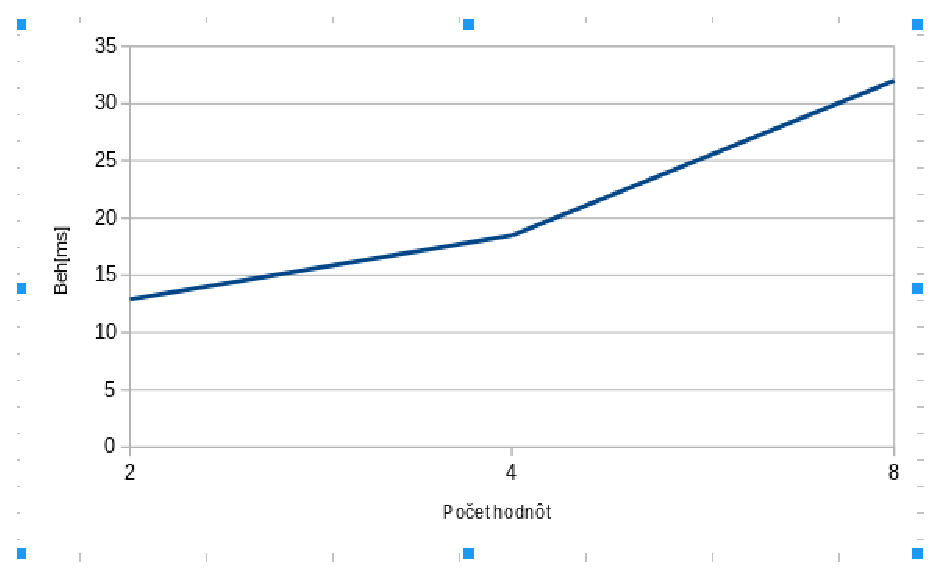
\includegraphics{img/mes.eps}}
\caption{Grap časovej závislosti behu programu v ms od počtu vstupných hodnôt}
\end{center}

\end{figure}





\section{Záver}
Implementovali sme algoritmus Minimum Extraction Sort s knižnicou OpenMPI jazykom C. Rovnako sme odvodili teoretickú časovú, priestorovú a celkovú zložitosť algoritmu. Zistili sme, že algoritmus nie je pre paralelné riešenie optimálny. V sekcii "Implementácia" som vysvetlil svoje riešenie pre tento algoritmus. Celkový flow akým spôsobom sú dáta preposielané medzi jednotlivými procesormi je vysvetlený sekcii "Komunikačný protokol". Najdôležitejšou časťou celej dokumentácie je sekcia "Experimenty", v ktorej som overil svoje implementačné riešenie a zároveň potvrdil, že teoretická časová zložitosť odpovedá mojim experimentom.

\end{document}



